% !TEX program = xelatex
\documentclass[10pt,letterpaper,twocolumn]{article}

\usepackage[top=0.72in,bottom=0.72in,left=0.72in,right=0.72in]{geometry}
\usepackage{fontspec}
\setmainfont{Latin Modern Roman}[
  Extension=.otf,UprightFont=lmroman10-regular,BoldFont=lmroman10-bold,
  ItalicFont=lmroman10-italic,BoldItalicFont=lmroman10-bolditalic]
\setsansfont{Latin Modern Sans}[
  Extension=.otf,UprightFont=lmsans10-regular,BoldFont=lmsans10-bold,
  ItalicFont=lmsans10-oblique,BoldItalicFont=lmsans10-boldoblique]
\setmonofont{Latin Modern Mono}[Extension=.otf,UprightFont=lmmono10-regular,Scale=0.82]
\newfontfamily\acbold{ywft-processing-bold}[
  Path=../../system/public/type/webfonts/,Extension=.ttf]
\newfontfamily\aclight{ywft-processing-light}[
  Path=../../system/public/type/webfonts/,Extension=.ttf]

\usepackage{xcolor}
\usepackage{titlesec}
\usepackage{enumitem}
\usepackage{booktabs}
\usepackage{tabularx}
\usepackage{fancyhdr}
\usepackage{hyperref}
\usepackage{xurl}
\usepackage{graphicx}
\usepackage{microtype}
\usepackage{listings}
\usepackage[numbers,sort&compress]{natbib}
\usepackage{tikz}
\usetikzlibrary{arrows.meta,positioning,fit}

\definecolor{acpink}{RGB}{180,72,135}
\definecolor{acblue}{RGB}{44,92,188}
\definecolor{acred}{RGB}{190,48,62}
\definecolor{acdark}{RGB}{48,43,56}
\definecolor{acgray}{RGB}{105,105,110}
\definecolor{aclightgray}{RGB}{244,243,246}

\hypersetup{colorlinks=true,linkcolor=acblue,urlcolor=acblue,citecolor=acblue,
  pdfauthor={@jeffrey},
  pdftitle={Silent by Default: Four macOS Failure Modes That Disguise Microphone Capture as a Routing Bug}}
\titleformat{\section}{\normalfont\bfseries\normalsize\uppercase}{\thesection.}{0.45em}{}
\titlespacing{\section}{0pt}{1.15em}{0.3em}
\titleformat{\subsection}{\normalfont\bfseries\small}{\thesubsection}{0.45em}{}
\titlespacing{\subsection}{0pt}{0.8em}{0.2em}
\pagestyle{fancy}
\fancyhf{}
\renewcommand{\headrulewidth}{0pt}
\fancyhead[C]{\footnotesize\color{acpink}\textit{silent by default --- system report}}
\fancyfoot[C]{\footnotesize\thepage}
\setlist[itemize]{nosep,leftmargin=1.2em,itemsep=0.1em}
\setlength{\columnsep}{1.7em}
\setlength{\parindent}{1em}
\setlength{\parskip}{0.25em}
\makeatletter
\setlength{\@fptop}{0pt}
\setlength{\@dblfptop}{0pt}
\makeatother
\tolerance=900
\emergencystretch=1em
\graphicspath{{../arxiv-ac/figures/}}
\newcommand{\ac}{\textsc{Aesthetic.Computer}}
\newcommand{\app}{\textsc{DubWizard}}
\newcommand{\code}[1]{\texttt{#1}}

\lstset{basicstyle=\ttfamily\scriptsize,breaklines=true,frame=single,
  showstringspaces=false,columns=fullflexible,keepspaces=true,
  rulecolor=\color{acgray!30},backgroundcolor=\color{aclightgray},
  xleftmargin=0.4em,xrightmargin=0.4em,aboveskip=0.5em,belowskip=0.5em}

\begin{document}

\twocolumn[{%
\begin{center}

\includegraphics[height=3.5em]{pals}\par\vspace{0.45em}
{\acbold\fontsize{21pt}{25pt}\selectfont\color{acdark} Silent by Default}\par
\vspace{0.2em}
{\aclight\fontsize{12pt}{14pt}\selectfont\color{acpink}
  Four macOS Failure Modes That Disguise Microphone Capture as a Routing Bug}\par
\vspace{0.55em}
{\normalsize\href{https://prompt.ac/@jeffrey}{@jeffrey}}\par
{\small\color{acgray} Aesthetic.Computer --- 8 August 2026}\par
{\small\color{acgray} ORCID: \href{https://orcid.org/0009-0007-4460-4913}{0009-0007-4460-4913}}\par
\vspace{0.35em}
{\small\color{acblue}\url{https://aesthetic.computer}}\par
\vspace{0.55em}\rule{\textwidth}{1.5pt}\vspace{0.35em}
\end{center}

\begin{quote}
\small\noindent\textbf{Abstract.}
A vocal-dub recorder for \ac{} could not capture from a Focusrite Scarlett Solo. The symptom set --- an armed monitor that stayed silent, a window that never appeared, and an intermittent startup abort --- read as an audio-routing problem, and an extended automated session pursued it as one, repeatedly re-routing devices without resolution. This report documents the differential diagnosis that followed. Four independent faults were operating at once, and only one concerned routing. First, \code{AVAudioEngine} binds a single Core Audio HAL unit to both its input and its output, making the intended ``built-in microphone in, interface out'' topology impossible on one engine; the constraint is directly observable as \code{inputNode.audioUnit == outputNode.audioUnit}. Second, no connection from the input node to any mixer existed, so monitoring could never have been audible regardless of device. Third, instantiating the engine's I/O unit blocks inside \code{AudioComponent\allowbreak Instance\allowbreak New} while a Transparency, Consent, and Control (TCC) microphone prompt is pending --- through either node --- which on the main thread freezes the window at $0\times0$ and presents as ``the app has no interface'' rather than ``the app is waiting on you.'' Fourth, the permission itself could never persist, because an ad-hoc code signature is identified by its \code{cdhash} and every rebuild therefore appeared to macOS as a distinct application. We give a reproducible probe method, the corrected implementation, and a signing and bundling recipe under which the grant survives rebuilds. End-to-end capture remains unverified pending a single user consent action, and we state that limit rather than claim a fix we did not observe.
\end{quote}
\vspace{0.4em}
}]

\section{The Problem}

\app{} is a small Swift application in the \ac{} workspace that plays a finished mix through an audio interface while recording free-form vocal takes against it, indexing each take by timeline position for later curation. It is a companion to \textsc{WaveWizard}, which teaches notes; \app{} captures performance.

Its first implementation could not record. The reported symptoms were three, and they appeared unrelated:

\begin{itemize}
  \item \textbf{Silent arming.} Engaging the monitor produced no audible signal and no level indication, on any selected device.
  \item \textbf{No interface.} The application process was alive but presented no window and no Dock icon.
  \item \textbf{Intermittent aborts.} Some builds terminated during startup.
\end{itemize}

Each symptom independently suggests audio routing, and the preceding development session --- an automated agent session recorded in the workspace session ledger --- treated them that way for several hours. It set the system default input device, then reverted; it moved device detection off the main thread, then moved graph construction off as well; it removed a reverb node it believed was rejecting a format; it lowered the hardware buffer to 16 frames in pursuit of latency. Each change addressed a plausible cause. None resolved the symptom, and the session ended mid-repair.

The pattern is worth naming because it is not specific to this application. On contemporary macOS, a process denied microphone access does not receive an error. It receives buffers of zeros at the correct sample rate and channel count, indefinitely. Every downstream observable --- device enumeration, format negotiation, tap installation, callback cadence --- remains healthy. The failure is therefore indistinguishable, from inside the audio graph, from a correctly configured input with no signal on the wire. An engineer reading only audio-layer evidence will conclude the problem is routing, because routing is the only thing the audio layer can describe.

This report is a record of stepping outside that layer.

\section{Project Context}

\ac{} maintains a family of small native ``wizard'' applications alongside its browser runtime, and audio latency across those surfaces has been characterised previously \cite{scudderLatency}. The instrument work in \textsc{Notepat} \cite{scudderNotepat} and the native operating-system lane \cite{scudderOS} share the same constraint set: real hardware, low buffer targets, and a preference for observable state over convenience abstractions.

The relevant platform literature is Apple's own. \code{AVAudioEngine} is documented as a graph over a single I/O unit \cite{appleAVAudioEngine}; the Core Audio HAL exposes devices, streams, and buffer sizing through \code{AudioObject} properties \cite{appleCoreAudio}; and TCC governs microphone consent, with a hardened-runtime entitlement requirement for capture \cite{appleHardenedRuntime,appleMicPrivacy}. Each of the four faults below is consistent with that documentation. None of them is announced at runtime, which is the practical gap this report addresses.

A closely related precedent exists inside the same workspace: an earlier screen-capture subsystem required a stable code-signing identity so that TCC grants would survive rebuilds. That lesson had been recorded for screen recording and not generalised to audio. It applies identically.

\section{Method}

The diagnosis used differential probing: construct the smallest program that isolates one variable, run it under conditions that differ in exactly one respect, and compare. Four instruments were used.

\subsection{A standalone engine probe}

A single-file Swift program enumerated devices through the HAL, bound an engine to a chosen device, printed the negotiated formats, installed a tap, and reported per-channel peak amplitude over a fixed interval. Running it unbundled and then inside a signed application bundle isolates permission effects from routing effects, because only the bundle identity changes.

\subsection{A known-good external capture path}

\code{ffmpeg}'s \code{avfoundation} input provided an independent reader. Its \code{volumedetect} filter reports mean and maximum amplitude, which distinguishes ``no signal'' from ``zeros.''

\subsection{Process sampling}

\code{sample(1)} attributes wall-clock time to stack frames. Applied to a process presenting no window, it answers directly whether the main thread is blocked and where, without instrumenting the source.

\subsection{Direct TCC inspection}

The per-user TCC database records one row per (service, client) pair with an authorisation value and a code-signing requirement. Reading it distinguishes ``denied'' from ``never asked'' from ``asked under a different identity'' --- three states that produce identical audio-layer behaviour.

\section{Findings}

Table~\ref{tab:modes} summarises the four faults. Each was independently sufficient to produce silence.

\begin{table*}[t]
\centering
\small
\begin{tabularx}{\textwidth}{@{}p{3.5cm}p{3.6cm}X@{}}
\toprule
\textbf{Observed symptom} & \textbf{Apparent cause} & \textbf{Actual cause and correction} \\
\midrule
Interface input cannot be selected; wrong device appears active &
Device routing is not being applied &
One \code{AVAudioEngine} binds one HAL unit to \emph{both} directions. A split ``built-in in, interface out'' topology requires an aggregate device. Corrected by running the full-duplex interface for both. \\
\addlinespace
Arming the monitor is silent &
Input device selection is failing &
No connection existed from the input node to any mixer. Arming installed a metering tap only. Corrected by connecting input $\rightarrow$ EQ $\rightarrow$ monitor mixer $\rightarrow$ main mixer. \\
\addlinespace
No window; process alive with no Dock icon &
An AppKit activation or window-ordering defect &
The main thread was blocked in \code{AudioComponent\allowbreak Instance\allowbreak New} awaiting a pending TCC prompt. Corrected by performing no audio work until the grant resolves. \\
\addlinespace
Microphone grant appears present but capture returns zeros &
A Core Audio or device fault &
Ad-hoc signatures are identified by \code{cdhash}, so each rebuild is a new application to TCC. Corrected by Developer ID signing with a bound identifier. \\
\bottomrule
\end{tabularx}
\caption{Four concurrent faults. Only the first concerns routing; all four present as routing failures because a permission-denied input is indistinguishable from a correctly configured silent one.}
\label{tab:modes}
\end{table*}

\subsection{One engine binds one device}

The intended topology --- capture from the built-in microphone, play out through the interface --- cannot be expressed with a single \code{AVAudioEngine} on macOS. The engine's input and output are two ends of one Audio Unit HAL (AUHAL) instance. The probe makes this checkable in one line, and it evaluates true:

\begin{lstlisting}[language=Swift]
engine.inputNode.audioUnit == engine.outputNode.audioUnit  // true
\end{lstlisting}

Consequently \code{kAudioOutputUnit\allowbreak Property\allowbreak\_CurrentDevice} is not an input-side or output-side setting; it is \emph{the} device for the engine. Setting it for playback silently redefines capture as well. Splitting the directions requires an aggregate device, which introduces a second clock domain and its own drift handling.

The practical resolution is simpler than the workaround: the interface in question is full duplex. Table~\ref{tab:devices} shows the inventory as the corrected enumerator reports it. The Scarlett Solo presents two input and two output channels at 48\,kHz and can carry playback and capture on one clock, which is both the lowest-latency arrangement and the one an audio interface exists to provide.

\begin{table}[t]
\centering
\small
\begin{tabular}{@{}lrrl@{}}
\toprule
\textbf{Device} & \textbf{In} & \textbf{Out} & \textbf{Mode} \\
\midrule
Scarlett Solo USB & 2 & 2 & full duplex \\
BlackHole 2ch & 2 & 2 & full duplex \\
ZoomAudioDevice & 2 & 2 & full duplex \\
MacBook Neo Microphone & 1 & 0 & input only \\
aesthetic.computer Microphone & 1 & 0 & input only \\
MacBook Neo Speakers & 0 & 2 & output only \\
\bottomrule
\end{tabular}
\caption{Device inventory after correcting the channel count, which previously read only the first buffer of the \code{AudioBufferList} and undercounted any device publishing channels non-interleaved.}
\label{tab:devices}
\end{table}

Once the device is bound before any format is read, the input side reports the interface correctly --- 48\,kHz, two channels --- matching the HAL's own stream description. Routing, in other words, was never broken. It merely had to be established in an order Core Audio tolerates: bind the device, then read formats, then connect, then prepare.

\subsection{The monitor path did not exist}

The original implementation declared a monitor mixer, a parametric equaliser, and a reverb, and attached none of them. Engaging \textsc{arm} installed a tap on the input bus and set a gain value on an unattached node. A tap is a capture facility; it does not route audio anywhere. No edge connected the input node to the main mixer, so no configuration of devices or permissions could have made monitoring audible.

This fault is invisible to device-level debugging and explains why every routing change appeared to fail. Figure~\ref{fig:graph} shows the corrected graph.

\begin{figure}[t]
\centering
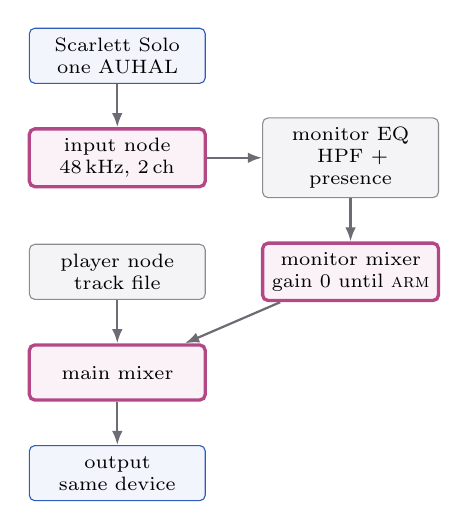
\begin{tikzpicture}[
  node distance=5.5mm and 7mm,
  box/.style={draw=acdark!55,rounded corners=2pt,fill=aclightgray,
    align=center,minimum height=7mm,text width=20mm,font=\scriptsize},
  core/.style={box,draw=acpink,very thick,fill=acpink!7},
  hw/.style={box,draw=acblue,fill=acblue!6},
  arrow/.style={-{Latex[length=1.8mm]},thick,draw=acdark!70}]
  \node[hw] (dev) {Scarlett Solo\\one AUHAL};
  \node[core,below=of dev] (in) {input node\\48\,kHz, 2\,ch};
  \node[box,right=of in] (eq) {monitor EQ\\HPF + presence};
  \node[core,below=of eq] (mix) {monitor mixer\\gain 0 until \textsc{arm}};
  \node[box,left=of mix] (play) {player node\\track file};
  \node[core,below=of play] (main) {main mixer};
  \node[hw,below=of main] (out) {output\\same device};
  \draw[arrow] (dev)--(in);
  \draw[arrow] (in)--(eq);
  \draw[arrow] (eq)--(mix);
  \draw[arrow] (mix)--(main);
  \draw[arrow] (play)--(main);
  \draw[arrow] (main)--(out);
\end{tikzpicture}
\caption{The corrected graph. The three edges from the input node through the monitor chain to the main mixer were absent in the original; arming set a gain on a node that was never attached.}
\label{fig:graph}
\end{figure}

\subsection{Engine construction blocks on a pending prompt}

The missing window was the most misleading symptom, and it was not an AppKit fault. Sampling the process attributed every sample of the main thread to a single blocked call:

\begin{lstlisting}
2213 DubSession.rebuild(with:includeInput:)
 2213 Hardware.bindEngine(_:to:)
  2213 -[AVAudioEngine inputNode]
   2213 AVAudioEngineImpl::UpdateInputNode(bool)
    2213 AVAudioEngineImpl::GetIOUnit(bool, AVAudioSession*)
     2213 AVAudioIOUnit::Create(...)
      2213 AudioComponentInstanceNew
       2213 ... (in CoreAudio)
\end{lstlisting}

All 2213 of 2213 samples. Instantiating the engine's I/O unit blocks until the user answers the microphone prompt. Performed on the main thread during \code{application\allowbreak DidFinish\allowbreak Launching}, it prevents the run loop from ever laying out the window, which is then reported by the window server at zero size and off screen.

An initial correction deferred only the input-side format read. This was insufficient: the block recurred through \code{outputNode}, because \code{GetIOUnit} creates the unit with input enabled regardless of which node requests it. The sample after that change showed 1526 of 1526 samples in \code{UpdateOutputNode} reaching the same \code{AudioComponent\allowbreak Instance\allowbreak New}. The correct rule is stronger than deferring input: \emph{no} \code{AVAudioEngine} construction may precede the consent decision. Once TCC has decided --- granted or denied --- instantiation no longer blocks, so the graph is safe to build in the completion handler.

Table~\ref{tab:window} records the effect. The application had been described across an entire prior session as having no user interface; it had a user interface throughout, and was waiting.

\begin{table}[t]
\centering
\small
\begin{tabular}{@{}lll@{}}
\toprule
\textbf{Build} & \textbf{Window bounds} & \textbf{On screen} \\
\midrule
Audio graph before consent & $0\times0$ at $(0,0)$ & no \\
Input read deferred only & $0\times0$ at $(0,0)$ & no \\
All audio after consent & $468\times346$ at $(470,177)$ & yes \\
\bottomrule
\end{tabular}
\caption{Window geometry reported by the window server. The interface was never defective; the main thread was blocked before layout could occur.}
\label{tab:window}
\end{table}

\subsection{The grant could not persist}

Three separate consent conditions were violated, each producing silence without a diagnostic.

\textbf{Location.} A bundle placed under \code{/private/tmp} received no prompt and no database row; the access request simply returned false. Moving the identical bundle to \code{\textasciitilde/Applications} restored prompting behaviour.

\textbf{Entitlement.} Signed with the hardened runtime but without \code{com.apple.\allowbreak security.\allowbreak device.\allowbreak audio-input}, the request was denied outright with no dialog. Adding the entitlement restored the prompt.

\textbf{Signature stability.} This is the fault that made the problem recur indefinitely. The original bundle was ad-hoc signed:

\begin{lstlisting}
Identifier=DubWizard-5555494461c95d69...
Signature=adhoc
Info.plist=not bound
Sealed Resources=none
\end{lstlisting}

An ad-hoc signature carries no team identity, so TCC binds the grant to the binary's \code{cdhash}. Every rebuild changes that hash, so every rebuild is a different application to the consent system --- while the database still shows a row for the bundle identifier, reading as though permission were held. Re-signing with a Developer ID identity and an explicit \code{--identifier} pins identity to team and bundle identifier, and the grant survives rebuilds.

The transition has a one-time cost that is worth stating plainly: changing the signature invalidates any existing row, after which \code{authorizationStatus} reports \code{notDetermined} even though the stored value still reads as authorised. A single \code{tccutil reset} clears the stale row so consent can be granted once against the stable identity.

\section{Implementation}

The corrected application makes the diagnosis structural rather than remembered.

\textbf{Ordered binding.} Device selection, format reading, connection, and preparation occur in the one order Core Audio accepts, and the bound device is read back and verified rather than assumed.

\textbf{Whole-graph rebuild.} Changing devices discards the engine and constructs a new one. \code{AVAudioEngine} caches the format observed at connect time; reusing a graph across a device change is what produced the startup abort, which the crash report attributes to \code{AVAudioEngine\allowbreak Graph::\allowbreak\_Connect} raising through \code{objc\_\allowbreak exception\_\allowbreak rethrow} to \code{abort()}.

\textbf{Buffer sizing.} The hardware buffer and \code{maximum\allowbreak Frames\allowbreak To\allowbreak Render} are 128 frames, roughly $2.7$\,ms at 48\,kHz. The previous target of 16 frames is below what the interface accepts and left the graph in a state that aborted on connect. The pursuit of 16 frames was a latency optimisation applied before the signal path worked at all.

\textbf{Per-channel metering.} The interface's channels are metered independently and displayed. On this device, channel one is the XLR microphone input and channel two is the instrument jack. A dead channel one is therefore visible as a dark meter, which distinguishes absent phantom power or a closed gain stage --- physical conditions no software change can repair --- from a routing or permission fault.

\textbf{Consent-first startup.} The window is presented, the consent decision is awaited, and only then is any audio object constructed.

\textbf{A headless level check.} \code{--meter} binds an input and reports per-channel peaks without the interface, so signal presence can be established non-interactively.

\textbf{A signing recipe.} A build script produces the bundle in a normal location, signs it with Developer ID and a bound identifier, and attaches the audio-input entitlement. Its comments record why each element is load-bearing, since all three fail silently.

\section{Evidence}

The distinguishing measurement is the amplitude signature of a denied input. Reading the built-in microphone from an unentitled process reported a mean and maximum volume of $-91.0$\,dB across 22\,016 samples, with the entire histogram in a single bin --- the signature of exact zeros rather than a quiet room. The engine probe reported per-channel peaks of $0.00000$ on both interface channels under the same conditions. Identical readings from two independent capture paths, on two different devices, established that the silence was upstream of the audio graph.

Two conditions were confirmed separately: consent state, by direct inspection of the TCC database before and after each signing change; and main-thread blocking, by process sampling, which localised the stall to a single call and later confirmed that the first correction had not removed it.

Verified after the rewrite: the application builds and starts without the abort, device enumeration reports the interface as full duplex with correct channel counts, the bound device reads back as requested, the negotiated input format matches the HAL stream description, and the window renders on screen at its intended size.

Not verified: end-to-end capture of an acoustic signal. The consent dialog raised by the corrected build remained unanswered at the time of writing --- the display was locked for part of the session, and macOS both queues prompts behind the lock screen and zeroes microphone capture while locked, which invalidated several earlier readings. The remaining step is a single consent action, after which the per-channel meters or the headless check will establish whether signal is present on the XLR channel. We record this as unfinished rather than assert a repair we did not observe.

\section{Ethics, Privacy, and Limitations}

The consent mechanisms described here are privacy controls, and nothing in this report is a means of circumventing them. Every correction moves in the opposite direction: toward requesting consent properly, at a stable identity the user can recognise and later revoke, and toward surfacing the permission state in the interface instead of letting it present as a hardware defect. The one destructive-sounding operation, \code{tccutil reset}, revokes a grant and forces a fresh prompt; it does not confer access. A user who does not consent gets a functioning playback-only application and an explicit statement of why capture is unavailable.

The findings are limited in scope. They were established on a single machine --- macOS 26.5.2 on Apple silicon, Swift 6.3.3, with one class of USB interface --- and the blocking behaviour of \code{AudioComponent\allowbreak Instance\allowbreak New} under a pending prompt is an observed runtime property, not a documented contract, so it may vary across releases. The aggregate-device path for split input and output topologies was reasoned about but not implemented or measured. The latency figures quoted are buffer targets rather than measured round-trip times; the earlier report on input and audio latency \cite{scudderLatency} describes the measurement method that would be required to make a real claim. Finally, this is a report on one application's defects, and the generalisation we draw --- that permission-denied audio is indistinguishable from configured-but-silent audio --- is offered as a diagnostic heuristic rather than a proven property of the platform.

\section{Conclusion}

Four faults produced one symptom, and the symptom pointed at the only layer that could describe it. The engine could not hold the intended topology, the monitor path was never connected, construction blocked on an unanswered prompt, and the permission could not persist across a rebuild. Three of the four had nothing to do with audio routing, and all three were invisible to audio-layer instrumentation.

What resolved it was not a better hypothesis about routing but a change of instrument: a signed bundle to isolate consent from configuration, an external reader to characterise the silence, a process sample to locate the block, and the consent database read directly rather than inferred. The generalisable lesson is narrow and practical. When a macOS audio input is silent, establish the consent state before reasoning about the graph --- the platform will not tell you, and every other observable will look correct while it lies.

The corrective principle is equally narrow: build no audio object until consent is decided, connect the monitor path explicitly, bind one device for both directions unless an aggregate is genuinely required, and sign with a stable identity so the grant outlives the build.

\section{Reproduction}

The diagnosis reduces to five commands, in the order that separates consent from configuration. Each answers one question the audio graph cannot.

\begin{lstlisting}[language=bash]
# 1. Which devices exist, and which are full duplex?
DubWizard --list-devices

# 2. Is the input consented, denied, or never asked?
cd ~/Library/Application\ Support/com.apple.TCC
sqlite3 TCC.db "select client, auth_value from \
  access where service='kTCCServiceMicrophone'"

# 3. Characterise the silence independently.
#    A flat -91 dB histogram means exact zeros,
#    which is denial -- not a quiet room.
ffmpeg -f avfoundation -i ":1" -t 3 \
  -af volumedetect -f null -

# 4. Is the main thread blocked, and where?
sample $(pgrep DubWizard) 3

# 5. Per-channel levels, no interface needed.
DubWizard --meter scarlett --out=/tmp/meter.txt
\end{lstlisting}

\noindent Step 2 is the one most often skipped, and it is the one that reorders everything after it. A row whose authorisation value reads as granted is not sufficient evidence of access: if the signing identity has changed since the row was written, the stored requirement no longer matches and the effective state is \code{notDetermined} while the database still reads as authorised.

\vspace{0.6em}
\noindent\textbf{Availability.} Source, build script, and the headless meter mode are in the \ac{} repository under \code{wave-wizard/}, commit \code{11546b593}.

\small
\begin{thebibliography}{9}

\bibitem{scudderLatency}
J. Scudder, ``Where the Microseconds Go: Input and Audio Latency in AC Native OS,'' Aesthetic Computer Papers, 2026. \url{https://papers.aesthetic.computer/latency}

\bibitem{scudderNotepat}
J. Scudder, ``Notepat,'' Aesthetic Computer Papers, 2026. \url{https://papers.aesthetic.computer/notepat}

\bibitem{scudderOS}
J. Scudder, ``Aesthetic Computer as an Operating System,'' Aesthetic Computer Papers, 2026. \url{https://papers.aesthetic.computer/os}

\bibitem{appleAVAudioEngine}
Apple Inc., ``AVAudioEngine,'' AVFAudio framework documentation. \url{https://developer.apple.com/documentation/avfaudio/avaudioengine}

\bibitem{appleCoreAudio}
Apple Inc., ``Core Audio: Audio Hardware Services and AudioObject properties,'' Core Audio framework documentation. \url{https://developer.apple.com/documentation/coreaudio}

\bibitem{appleHardenedRuntime}
Apple Inc., ``Hardened Runtime: resource access entitlements,'' Developer documentation. \url{https://developer.apple.com/documentation/security/hardened_runtime}

\bibitem{appleMicPrivacy}
Apple Inc., ``Requesting authorization to capture and save media,'' AVFoundation documentation. \url{https://developer.apple.com/documentation/avfoundation/requesting-authorization-to-capture-and-save-media}

\bibitem{repo}
Aesthetic Computer contributors, ``DubWizard source, ring buffer, and bundling script,'' \code{wave-wizard/}, commit \code{11546b593}, 8 August 2026. \url{https://github.com/whistlegraph/aesthetic-computer}

\end{thebibliography}

\end{document}
